%! TEX program = lualatex

\documentclass[journal,twoside,web]{ieeecolor}

\usepackage{generic}
%/========== Preamble ==========/%
% Packages required by ieeecolor
\usepackage{amsmath}
\usepackage{amsfonts}
\usepackage{amssymb}
\usepackage{algorithmic}
\usepackage{graphicx}
\usepackage{subcaption}
\usepackage{textcomp}
\usepackage{cite}

%---------- More packages ----------%
% NOTE: cannot use amsthm for some reason
\usepackage{mathtools}
\usepackage{bm}

%---------- Bibliography Style ----------%
\bibliographystyle{IEEEtran}

%---------- Header ----------% 
\newcommand*{\Title}{VNHC and Acrobot Title}
\markboth{\journalname, VOL. XX, NO. XX, XXXX 2021}
{Moran-MacDonald \MakeLowercase{\textit{et al.}}: \Title}

%---------- Theorems ----------%
\newtheorem{thm}{Theorem}% Uncomment: reset numbering at each chapter
\newtheorem{prop}[thm]{Proposition} % Propositions depend on Theorem number
\newtheorem{lemma}[thm]{Lemma} % Same with lemmas
\newtheorem{defn}[thm]{Definition} % Definitions depend on theorem number
\newtheorem{assm}{Assumption} % Assumptions do not reset 

%---------- Special Commands ----------%
\DeclarePairedDelimiter{\norm}{\lVert}{\rVert}
\DeclarePairedDelimiter{\abs}{\lvert}{\rvert}
\DeclareMathOperator{\Rank}{rank}
\DeclareMathOperator{\Sign}{sgn}
\DeclareMathOperator{\Diag}{diag}
\newcommand*{\rank}[1]{\Rank\left(#1\right)}
\newcommand*{\sign}[1]{\Sign\left(#1\right)}
\newcommand*{\diag}[1]{\Diag\left(#1\right)}

\newcommand*{\tpose}{^\mathsf{T}} 
\newcommand*{\inv}{^\mathsf{-1}}
\newcommand*{\Rt}[1]{[\R]_{#1}}
\newcommand*{\R}{\mathbb{R}}
\newcommand*{\n}{\mathbf{n}}
\newcommand*{\N}{\mathbb{N}}
\newcommand*{\Sone}{\mathbb{S}^1}
\newcommand*{\SxR}{\Sone \times \R}
\newcommand*{\Minv}{M^\mathsf{-1}}
\newcommand*{\Id}[1]{I_{#1}}
\newcommand*{\Zmat}[1]{\bm{0}_{#1}}
\newcommand*{\diff}[2]{\frac{d #1}{d #2}}
\newcommand*{\ddiff}[3]{\frac{d^2 #1}{d #2 d #3}}
\newcommand*{\pdiff}[2]{\frac{\partial #1}{\partial #2}}

\newcommand*{\simpleB}{\begin{bmatrix}\Zmat{(n-k)\times k}\\ \Id{k}\end{bmatrix}}
\newcommand*{\pdmat}{(\Id{n} \otimes p\tpose)\nabla_q\Minv(q)p}
\newcommand*{\pudmat}{(\Id{n-k} \otimes p\tpose)\nabla_{q_u}\Minv(q)p}
%/========== /Preamble ==========/%

%/========== Main Document ==========/%
\begin{document}
\title{\Title}
\author{Adan Moran-MacDonald, \IEEEmembership{Member, IEEE}, Manfredi Maggiore
\IEEEmembership{Member, IEEE}*, and Xingbo Wang
\thanks{Manuscript submitted for review on \today.}
\thanks{A. Moran-MacDonald is with the Department of Electrical and Computer
    Engineering, University of Toronto, Toronto, ON, Canada (e-mail:
adan.moran@mail.utoronto.ca).}
\thanks{M. Maggiore is with the Department of Electrical and Computer
Engineering, University of Toronto, ON, Canada (e-mail:
maggiore@control.utoronto.ca).}
\thanks{X. Wang is with ??? (e-mail: ???).}
} %/author

\maketitle

%/========== Abstract ==========/%
\begin{abstract}
TODO: Abstract here.
\end{abstract}

\begin{IEEEkeywords}
TODO: keywords in alphabetical order, separated by commas.
\end{IEEEkeywords}

%/========== Introduction ==========/%
\section{Introduction}\label{sec:introduction}
\IEEEPARstart{T}ODO: intro.

\subsection{Notation}
We use the following notation and terminology in this article.
A matrix \(A \in \R^{n \times m}\) is \textit{right semi-orthogonal} if
\(A A\tpose = \Id{n}\) and is \textit{left semi-orthogonal} if 
\(A\tpose A = \Id{m}\).
For \(A \in \R^{n\times m}\) and \(B \in \R^{p \times m}\),
we define \([A;B] \in \R^{(n+p)\times m}\) as the matrix obtained by stacking \(A\)
on top of \(B\). 
For \(T > 0\), the set of real numbers modulo \(T\) is denoted \(\Rt{T}\), with
\(\Rt{\infty} := \R\).
The gradient of a matrix-valued function 
\(A : \R^m \rightarrow \R^{n\times n}\) is the block matrix of stacked partial
derivatives, 
\(\nabla_xA := [\pdiff{A}{x_1};\ldots;\pdiff{A}{x_m}] \in \R^{nm \times n}\).
Given two matrices \(A \in \R^{n \times m}\) and \(B \in \R^{r \times s}\), the
Kronecker product \cite{kronprod} \(A \otimes B \in \R^{nr \times ms}\) is the
matrix
\begin{equation}\label{eqn:kronprod}
    A \otimes B = \begin{bmatrix}
        A_{1,1}B & \cdots & A_{1,m} B \\
        \vdots & \ddots & \vdots \\
        A_{n,1} B & \cdots & A_{n,m} B
    \end{bmatrix} 
    .
\end{equation}
The Poisson bracket \cite{landau_mechanics} between the functions
\(f(q,p)\) and \(g(q,p)\) is
\begin{equation}\label{eqn:poisson-bracket}
    [f,g] := \sum \limits_{i=1}^n \pdiff{f}{p_i}\pdiff{g}{q_i} - 
        \pdiff{f}{q_i}\pdiff{g}{p_i}
    .
\end{equation}
Finally, the Kronecker delta \(\delta_i^j = 1\) if \(i = j\) and \(0\)
otherwise.

%/========== Problem Formulation ==========/%
\section{Problem Formulation}\label{sec:problem-formulation}
%TODO: motivate injection/dissipation for energy regulation in an acrobot. Use
%this to lead into VNHCs. e.g. represent torso as chain of a swing, pivot as
%seat, and legs as human legs. Replicate fig3.3 from thesis but for acrobot: take
%(qu,pu)-plane and show how a person moves their legs wrt theta, qu, or pu. Leave
%the gymnast model until the end, or ignore it entirely.
%
%Alternatively, ff human movement journal says legs move wrt qu, we can use that
%as a foundation.
%Ideas: Human movement says appropriate regulation of pendulum allows energy to
%be pumped into system. Pendulum length rapidly increased on downward swing, then
%rapidly decreased on upward swing (I think these mean backward and forward).
%They plot pendulum length rdot/r vs "body angle" theta to determine energy
%injection, which hints at some relationship between (r,rdot) and (theta,thetad).
%Indeed, the peak value of rdot/r did not occur at a fixed value of theta, nor
%once anyone reached a particular speed; it occured at the same thetadot/theta for all
%participants of the study. This perfectly motivates VNHCs for robots, because we
%can shape (r,rtdot) as functions of (theta,thetad).
%Start motivation from energy injection - how do humans inject energy? How does
%acrobot model gymnast? use human movement to motivate tracking functions of both
%position and velocity rather than time.

In gymnastics terminology, a ``giant" is the motion a gymnast performs to
achieve full rotations around a horizontal bar \cite{usagym_giant}. 
A gymnast will begin by hanging at rest, then swing their legs
appropriately to gain energy over time.
The authors of \cite{pendulum_length_giant_gymnastics} modelled the gymnast as a
variable length pendulum, and studied how the pendulum's length changes as a
function of the gymnast's limb angle.
Labeling the pendulum length by \(r\) and the gymnast's body orientation
by \(\theta\), they observed experimentally that the value \(\dot{r}/r\) has
the biggest impact on the magnitude of energy injection. 
After testing several gymnasts under a variety of experimental conditions, 
they discovered that the peak value of \(\dot{r}/r\) occured at the same fixed
value of \(\dot{\theta}/\theta\) for all gymnasts.
In other words, gymnasts appear to move their legs as a function of their body
angle and velocity when performing giants; 
doing so allows them to gain energy and rotate around the bar.

While the simplest model of a gymnast is the variable-length pendulum, a
more realistic model is the two-link acrobot (Figure \ref{fig:acrobot}).
Here, the top link represents the torso, while the bottom link represents
the legs. 
The acrobot is actuated exclusively at the center joint (the hips).
Controlling the acrobot is a nontrivial task because it is not feedback
linearizable \cite{nonlinear_controllers_nonintegrable_acrobot}. 
To solve the swingup problem, one might begin by designing a leg controller
which provably injects energy into the acrobot, so that the resulting motion
mimics that of a human performing a giant.

\begin{figure}
    \centering
    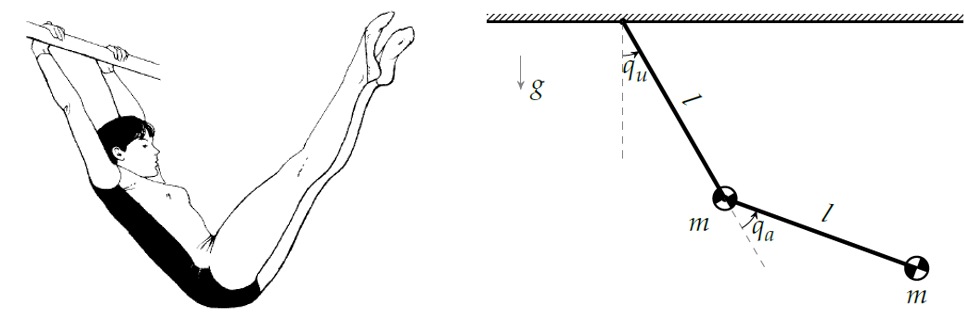
\includegraphics[width=\linewidth]{acrobot_gymnast.png}
    \caption{The two-link acrobot as a model for a gymnast.
    Image modified from \cite{xingbo_thesis}.}
    \label{fig:acrobot}
\end{figure}

Previous attempts at acrobot giant generation have involved
trajectory tracking, partial feedback linearization, or other energy-based
methods
( see
\cite{energy_pumping_robotic_swinging,swingup_giant_acrobot,dynamical_servo_acrobot_vc,control_giant_two_link_gymnastic_robot}
).
While all these approaches succeed at making the acrobot rotate around the
bar, none of them use the results of \cite{pendulum_length_giant_gymnastics}.
That is, none of these leg controllers track a function of the acrobot's body
angle and velocity.
In 2016, Wang attempted to design a controller which does this \cite{xingbo_thesis}
but was unable to prove the acrobot would gain energy over time.
His approach was a rudimentary version of a recent technique know as the method
of virtual nonholonomic constraints.

Virtual nonholonomic constraints (VNHCs) have been used for human-robot interaction
\cite{vnhc_human_robot_cooperation,psd_based_vnhc_redundant_manipulator,haptic_vnhc},
error-reduction on time-delayed systems \cite{vnhc_time_delay_teleop},
and they have shown marked improvements to the field of bipedal locomotion 
\cite{nhvc_dynamic_walking,
hybrid_zero_dynamics_bipedal_nhvcs,output_nhvc_bipedal_control}.
Indeed, they produce more robust walking motion in biped robots than
other controllers which do not depend on velocity \cite{nhvc_incline_walking}.
In particular, VNHCs may be capable of injecting and
dissipating energy from a system in a robust manner, all while producing
realistic biological motion. 

In this article, we will design a virtual
nonholonomic constraint which provably injects energy into the acrobot through 
human-like giant motion.

Before embarking on our design problem, let us summarize the relevant theory of
VNHCs.

%/========== VNHC ==========/%
\section{Theory of VNHCs}\label{sec:vnhc}

\subsection{Simply Actuated Hamiltonian Systems}
Take a mechanical system modelled with generalized coordinates 
\(q = (q_1, \ldots, q_n)\) on a configuration manifold
\(\mathcal{Q} = \Rt{T_1} \times \cdot \Rt{T_n}\), where
\(T_i = 2\pi\) if \(q_i\) is an angle and \(T_i = \infty\) if \(q_i\) is a
displacement. The corresponding generalized velocities are 
\(\dot{q} = (\dot{q}_1,\ldots,\dot{q}_n) \in \R^n\).

Suppose this system has Lagrangian
\(\mathcal{L}(q,\dot{q}) = 1/2~\dot{q}^T D(q) \dot{q} - P(q)\),
where the potential energy 
\(P : \mathcal{Q} \rightarrow \mathbb{R}\) 
is smooth, and the inertia matrix 
\(D : \mathcal{Q} \rightarrow \mathbb{R}^{n \times n}\)
is smooth and positive definite for all \(q \in \mathcal{Q}\).
The \textit{conjugate of momentum} to \(q\) is the vector
\(p := \partial\mathcal{L}/\partial\dot{q} = D(q) \dot{q} \in \R^n\).
As per \cite{landau_mechanics}, 
the \textit{Hamiltonian} of the system in \((q,p)\) coordinates
is
\begin{equation}\label{eqn:hamiltonian}
    \mathcal{H}(q,p) = \frac{1}{2} p\tpose D\inv(q) p + P(q)
    ,
\end{equation}
with dynamics
\begin{equation}\label{eqn:hamiltonian-eom-general}
    \begin{cases}
        \dot{q} = \nabla_p\mathcal{H} 
        , \\
        \dot{p} = -\nabla_q\mathcal{H} + B(q) \tau
        ,
    \end{cases}
\end{equation}
where \(\tau \in \R^k\) is a vector of generalized input forces and the input
matrix \(B : \mathcal{Q} \rightarrow \R^{n \times k}\) is full rank for all 
\(q \in \mathcal{Q}\).
If \(k < n\), we say the system is \textit{underactuated} with degree of
underactuation \((n-k)\).

It is easy to show using the matrix Kronecker product that
\eqref{eqn:hamiltonian-eom-general} expands to
\begin{equation}\label{eqn:hamiltonian-full-dynamics}
     \begin{cases}
        \dot{q} = D\inv(q)p 
        , \\
        \dot{p} = -\frac{1}{2} (\Id{n} \otimes p\tpose) \nabla_q D\inv(q) p
        - \nabla_q P(q) + B(q) \tau
        . \\
    \end{cases}
\end{equation}

Because \(\tau\) is transformed by \(B(q)\), it is not obvious how any
particular input force \(\tau_i\) affects the system.
As a first step in addressing this problem, we make the following assumptions.

\begin{assm}\label{assm:B-const}
    The input matrix \(B(q) \equiv B \in \R^{n\times k}\) is constant,
    full rank, and \(k < n\).
\end{assm}

\begin{assm}\label{assm:B-perp}
    There exists a right semi-orthogonal matrix 
    \(B^\perp \in \R^{(n-k)\times n}\)
    which is a left-annihilator for \(B\). 
\end{assm}

Note that Assumption \ref{assm:B-perp} requires the rows of \(B^\perp\) be unit vectors
that are mutually orthogonal. 
When \(k = (n-1)\), Assumption \ref{assm:B-perp} can be removed because it is
automatically implied by Assumption \ref{assm:B-const}.

The above assumptions allow us to define a
canonical coordinate transformation of ~\eqref{eqn:hamiltonian} 
which decouples the input forces.
To define this transformation we will make use of the following lemma.

\begin{lemma}\label{lemma:B-orthogonal}
    Suppose Assumption \ref{assm:B-const} holds. Then
    there exists a nonsingular matrix \(\hat{T} \in \R^{k \times k}\) 
    so that the regular feedback transformation 
    \[
        \tau = \hat{T} \hat{\tau}
    \] 
    has a new input matrix \(\hat{B}\) for \(\hat{\tau}\) which is left
    semi-orthogonal.  
\end{lemma}
\begin{proof}
    Since \(B\) is constant and full rank, it has a singular value decomposition 
    \(B = U\tpose \Sigma V\) where 
    \(\Sigma = [\diag{\sigma_1,\ldots,\sigma_k}; \Zmat{(n-k)\times k}]\),
    \(\sigma_i > 0\), and \(U \in R^{n \times n}\),
    \(V \in \R^{k \times k}\) are unitary matrices \cite{calculating_svd}.
    Defining \(T = \diag{1/\sigma_1^2,\ldots,1/\sigma_k^2}\) and assigning the
    regular feedback transformation \(\tau = V T \hat{\tau}\) yields a new input
    matrix \(\hat{B} = B V T\) for \(\hat{\tau}\) such that
    \(\hat{B}\tpose \hat{B} = T\tpose \Sigma\tpose \Sigma T = \Id{k}\).
\end{proof}

In light of Lemma \ref{lemma:B-orthogonal}, there is no loss of generality in
assuming that the input matrix is left semi-orthogonal.
Now, let \(\mathbf{B} := [B^\perp; B\tpose]\).
Since \(B^\perp\) is a left annihilator of \(B\) and both \(B^\perp\) and
\(B\tpose\) are right semi-orthogonal, one can easily show that \(\mathbf{B}\) is
an orthogonal matrix.

\begin{thm}\label{thm:simply-actuated}
    Take the Hamiltonian system ~\eqref{eqn:hamiltonian} and suppose
    Assumptions \ref{assm:B-const} and \ref{assm:B-perp} hold.
    The coordinate transformation
    \(\left(\tilde{q} = \mathbf{B}q, \tilde{p} = \mathbf{B}p\right)\)
    is a canonical transformation and the resulting dynamics are given by 
    \begin{gather}\label{eqn:simple-hamiltonian}
        \mathcal{H}(\tilde{q},\tilde{p}) = 
        \frac{1}{2} \tilde{p}\tpose \Minv(\tilde{q}) \tilde{p} + V(\tilde{q})
        , \\
       \begin{cases}
           \dot{\tilde{q}} = \Minv(\tilde{q})\tilde{p}
           , \\
           \dot{\tilde{p}} = -\frac{1}{2} (\Id{n} \otimes \tilde{p}\tpose)
           \nabla_{\tilde{q}} \Minv(\tilde{q}) \tilde{p} \\
           \phantom{---} - \nabla_{\tilde{q}} V(\tilde{q}) + \simpleB \tau
            ,
        \end{cases} \nonumber
    \end{gather}
    where 
    \(\Minv(\tilde{q}) := 
    \mathbf{B}D^{-1}(\mathbf{B}\tpose \tilde{q})\mathbf{B}\tpose\)
    and
    \(V(\tilde{q}) := P(\mathbf{B}\tpose \tilde{q})\).
\end{thm}
\begin{proof}
    Since \(\mathbf{B}\) is constant, this transformation satisfies
    \(\partial\tilde{q}_i/\partial p_j = \partial\tilde{p}_i/\partial q_j = 0\) for all 
    \(i,j \in \{1,\ldots,n\}\).
    This implies the Poisson brackets \([\tilde{q}_i, \tilde{q}_j]\)
    and \([\tilde{p}_i,\tilde{p}_j]\) are both zero.
    Then, since \(\mathbf{B}\) is orthogonal, 
    \([\tilde{p}_i, \tilde{q}_j] = (\mathbf{B}_i)\tpose (\mathbf{B}\tpose)_j
        = \delta_i^j\).
    By (45.10) in \cite{landau_mechanics}, this transformation is canonical and
    the new Hamiltonian is
    \(\mathcal{H}(\mathbf{B}\tpose \tilde{q}, \mathbf{B}\tpose \tilde{p})\).
    Finally, since \(\dot{\tilde{p}} = \mathbf{B} \dot{p}\), the input
    matrix for the system in \((\tilde{q},\tilde{p})\) coordinates is
    \(\mathbf{B}B = [\Zmat{(n-k)\times k}; \Id{k}]\), which proves the theorem.
\end{proof}

We call the \((\tilde{q},\tilde{p})\) coordinates
\textit{simply actuated coordinates}.
The first \((n-k)\) configuration variables in \(\tilde{q}\), labelled \(q_u\),
are the \textit{unactuated coordinates}; 
the remaining \(k\) configuration variables, labelled \(q_a\), are the
\textit{actuated coordinates}.
The corresponding \((p_u, p_a)\) in \(\tilde{p}\) are the \textit{unactuated}
and \textit{actuated momenta}, respectively.

\subsection{Virtual Nonholonomic Constraints}

The notion of a nonholonomic constraint which can be stabilized via state feedback
was first described by Griffin and Grizzle in \cite{nhvc_dynamic_walking}.
Horn et. al later extended their results in
\cite{hybrid_zero_dynamics_bipedal_nhvcs} and
derived the dynamics of constrained systems.
In this section we reformulate these ideas for the Hamiltonian framework,
because the theory is cleaner when using unactuated and actuated momenta.
For this reason, we take the system of inquiry to be a Hamiltonian
mechanical system in simply actuated coordinates, as in
\eqref{eqn:simple-hamiltonian}.
For simplicity of notation, we relabel \((\tilde{q},\tilde{p})\) as \((q,p)\).

\begin{defn}\label{defn:vnhc}
    A \textit{virtual nonholonomic constraint} (VNHC) \textit{of order \(k\)} is a
    relation \(h(q,p) = 0\) where \(h : \mathcal{Q}\times\R^n \rightarrow \R^k\) is
    \(C^2\), \(\rank{\left[ dh_q,\, dh_p \right]} = k\) for all 
    \((q,p) \in h\inv(0)\), and there exists a feedback controller \(\tau(q,p)\)
    rendering the \textit{constraint manifold} \(\Gamma\) invariant,
    where
    \begin{equation}
        \Gamma = \left\{(q,p) \mid h(q,p) = 0, dh_q \dot{q} + dh_p \dot{p} = 0\right\}
        .
    \end{equation}
\end{defn}

The constraint manifold is a \(2(n-k)\)-dimensional
closed embedded submanifold of \(\mathcal{Q} \times \R^n\).
A VNHC thereby allows us to study a reduced-order model of the system: it reduces
the original \(2n\) differential equations to \(2(n-k)\) equations.
In particular, if \(k = (n-1)\), the constraint manifold is \textit{always}
2-dimensional and its dynamics can be plotted on a plane. 

We often want to stabilize a constraint within some neighbourhood of \(\Gamma\).
To see when this is possible, let us define the error output \(e = h(q,p)\).
If any component of \(e_i\) has relative degree 1, we may not be able
to stabilize \(\Gamma\) -- we can always guarantee \(e_i \to 0\), but not
necessarily \(\dot{e}_i \to 0\).
It is for this reason that we define the following special type of VNHC.

\begin{defn}
    A VNHC \(h(q,p) = 0\) of order \(k\) is \textit{regular} if the output 
    \(e = h(q,p)\) is of relative degree \(\{2,2.\ldots,2\}\) everywhere on the
    constraint manifold \(\Gamma\).
\end{defn}

The authors of
\cite{nhvc_dynamic_walking,hybrid_zero_dynamics_bipedal_nhvcs}
observed that relations which use only the unactuated conjugate of momentum
often have vector relative degree \(\{2,\ldots,2\}\).
Indeed, we shall now provide a characterization of regularity which shows that
regular constraints cannot use the actuated momentum at all.

To ease notation in the rest of this section, we use the following shorthand:
\begin{align}
    \mathcal{A}(q,p_u) &:= dh_q(q,p_u) \Minv(q) 
        ,\\
    \mathcal{M}(q,p) &:= (\Id{n-k} \otimes p\tpose)\nabla_{q_u}\Minv(q) 
    .
\end{align}

\begin{thm}\label{thm:vnhc-regularity}
    A relation \(h(q,p) = 0\) for system ~\eqref{eqn:simple-hamiltonian}
    is a regular VNHC of order \(k\) if and only if 
    \(dh_{p_a} = \Zmat{k \times k}\) 
    and
    \[
        \rank{\left(\mathcal{A}(q,p_u) - dh_{p_u}\mathcal{M}(q,p)\right)\simpleB} = k
         ,
    \]
    everywhere on the constraint manifold \(\Gamma\).
\end{thm}
\begin{proof}
    Let \(e = h(q,p) \in \R^k\).
    If \(dh_{p_a} \neq \Zmat{k\times k}\) for some \((q,p) \in \Gamma\), 
    then \(\tau\) appears in \(\dot{e}\) and the VNHC is not of relative degree
    \(\{2,\ldots,2\}\). Suppose now that \(dh_{p_a} = \Zmat{k\times k}\).
    Then 
    \(\dot{e} = \mathcal{A}(q,p_u)p - 
     dh_{p_u}\left(1/2~\mathcal{M}(q,p)p + \nabla_{q_u}V(q)\right)\).
    Taking one further derivative provides
    \( \ddot{e} = (\star) - 
        dh_{p_u}\left(1/2~d/dt~\left(\mathcal{M}(q,p)p\right)\right) 
        + \mathcal{A}(q,p_u)[\Zmat{(n-k)\times k};\Id{k}] \tau\),
    where \((\star)\) is a continuous function of \(q\) and \(p\).
    One can further show that
    \(dh_{p_u}\left(1/2~d/dt~\left(\mathcal{M}(q,p)p\right)\right)
        = (\star) + dh_{p_u}\mathcal{M}(q,p)[\Zmat{(n-k)\times k};
        \Id{k}]\tau\).
    Hence,
    \[
       \ddot{e} = (\star) +
       \left(\mathcal{A}(q,p_u) - dh_{p_u}\mathcal{M}(q,p)\right) \simpleB \tau
        ,
    \]
    which we write as \( \ddot{e} = E(q,p) + H(q,p)\tau\) for appropriate \(E\)
    and \(H\).
    From the definition of regularity, the VNHC \(h\) is regular 
    when \(e\) is of relative degree \(\{2,\ldots,2\}\), which is true 
    if and only if the matrix premultiplying \(\tau\) is nonsingular, and hence
    that \(H\) is invertible. This proves the theorem.
\end{proof}

Under additional mild conditions (see \cite{vhcs_for_el_systems}), a regular VNHC of
order \(k\) can be stabilized by the output-linearizing phase-feedback
controller
\begin{equation}
    \tau(q,p) = -H\inv(q,p)\left(E(q,p) + k_p e + k_d \dot{e}\right)
    ,
\end{equation}
where \(k_p, k_d > 0\) are control parameters which can be tuned on the
resulting error dynamices \(\ddot{e} = -k_p e - k_d \dot{e}\).

In Section \ref{sec:acrobot} we will enforce a regular constraint on the
acrobot of the form \(h(q,p) = q_a - f(q_u,p_u)\), where the actuators track a
function of the unactuated variables.
Intuitively then, the constrained dynamics should be parameterized by \((q_u, p_u)\).
Unfortunately, \(\dot{q}_u\) depends on \(p_a\), and for general systems one
cannot solve explicitly for \(p_a\) in terms of \((q_u,p_u)\) because
the \(\dot{p}\) dynamics contains the coupling term 
\((\Id{n} \otimes p\tpose)\nabla_{q}M(q)p\). 

We now introduce an assumption which allows us to solve for \(p_a\) as a
function of \((q_u,p_u)\), which in turn allows us to find the constrained
dynamics.

\begin{assm}\label{assm:inertially-actuated}
The inertia matrix does not depend on the unactuated coordinates, so that 
\(\nabla_{q_u}M(q) = \Zmat{n(n-k) \times n}\).
\end{assm}

\begin{thm}\label{thm:zero-dynamics}
    Let \(\mathcal{H}\) be a mechanical system in simply actuated
    coordinates satisfying Assumption \ref{assm:inertially-actuated}. 
    Let \(h(q,p_u) = 0\) be a regular VNHC of order \(k\) with constraint
    manifold \(\Gamma\). Suppose that on \(\Gamma\) one can solve for
    \(q_a\) as a function \(q_a = f(q_u,p_u)\).
    Then the constrained dynamics are given by
    \begin{equation}\label{eqn:qpu-dynamics}
        \left.\begin{aligned}
                \dot{q}_u &= 
                \left[\Id{(n-k)} ~ \Zmat{(n-k) \times k}\right]
                \Minv(q)p \\
            \dot{p}_u &= -\nabla_{q_u}V(q) \\
            \end{aligned}{}\right|_{\begin{array}{c}
                q_a = f(q_u,p_u) \\ 
                p_a = g(q_u,p_u) \\
            \end{array}}
            ,
    \end{equation}
    where
    \begin{align}\label{eqn:g-qpu}
        &g(q_u,p_u) := 
        \left(\mathcal{A}(q,p_u)[\Zmat{(n-k)\times k};\Id{k}] \right)\inv 
        (dh_{p_u} \nabla_{q_u}V(q) \nonumber
        \\
        &- \mathcal{A}(q,p_u)[\Id{(n-k)};\Zmat{k \times(n-k)}]p_u
        \left.)\right|_{q_a = f(q_u,p_u)}
        .
    \end{align}
\end{thm}
\begin{proof}
    Setting \(e = h(q,p_u)\) and using Assumption
    \ref{assm:inertially-actuated}, we find that
    \(\dot{e} = \mathcal{A}(q,p_u)p - dh_{p_u}\nabla_{q_u}V(q)\).
    Notice that
    \(\mathcal{A}(q,p_u)p = \mathcal{A}(q,p_u)[\Zmat{(n-k)\times k}; \Id{k}]p_a
    + \mathcal{A}(q,p_u)[\Id{n-k};\Zmat{k \times (n-k)}] p_u\).
    Since \(h(q,p_u)\) is regular, \(\mathcal{A}(q,p_u)\) is invertible.
    Taking \(e = \dot{e} = 0\), solving for \(p_a\), and setting 
    \(q_a = f(q_u,p_u)\) completes the proof.
\end{proof}

We conclude this section by formalizing the notion of energy injection for
VNHCs.

\begin{defn}\label{defn:energy-gain}
    Let \(\mathcal{Q}\) be an
    \(n\)-dimensional smooth generalized cylinder.
    Let \(f : \mathcal{Q} \rightarrow \mathcal{Q}\times\R^n\) be a smooth vector
    field and let \(D \subset M\) be open.
    The system described by \(\dot{x} = f(x)\) 
    \textit{gains energy on \(D\)} if, 
    for all compact sets \(K \subset D\) and for almost every initial
    condition \(x(0) \in K\), there exists \(T > 0\) such
    that \(x(t) \notin K \, (\forall t > T)\).
    The system \textit{loses energy on \(D\)} if it gains energy in
    negative-time.
\end{defn}

Any system satisfying Definition \ref{defn:energy-gain}
can have unstable equilibria on \(D\), but not limit cycles nor closed orbits.
The next definition ties this notion of energy gain to VNHCs.

\begin{defn}\label{defn:energy-injection}
    A regular VNHC \(h(q, p) = 0\) with constraint manifold \(\Gamma\)
    \textit{injects (dissipates) energy on \(D \subset \Gamma\)} if the
    constrained dynamics gain (lose) energy everywhere on \(D\), except possibly
    on a set of measure zero.
\end{defn}

\textbf{Comparison with existing literature}: Horn et.al. provide the constrained
dynamics for VNHCs in \cite{nhvc_incline_walking}.
Their assumption \textbf{H2} is what we call regularity, and our requirement
that one can solve for \(q_a = f(q_u,p_u)\) on \(\Gamma\) implies their
assumption \textbf{H3} holds true.
The only real distinction between this section and their work
is that our constrained dynamics are explicit functions of the Hamiltonian phase
coordinates \((q_u,p_u)\).
In fact, our constrained dynamics \eqref{eqn:qpu-dynamics} coincide with their
system (17) when one chooses the special case \(\theta_1 = q_u\) and 
\(\theta_2 = p_u\).
This explicit representation will be beneficial when we apply the theory of
VNHCs to the acrobot.

%/========== Acrobot ==========/%
\section{The Acrobot VNHC}\label{sec:acrobot}
%specialize the theory of VNHCs to the acrobot. consider constraints which depend
%only on pu, and show arctan vnhc and reduced dynamics. 
%give definition of energy injection/dissipation. conclude with our
%theorem. Make this section short and sweet.
%
%TODO: after writing S2, re-introduce what we want to do with acrobot (energy
%injection for giant stabilization)
Our goal in this article isto design a VNHC which injects energy into the
acrobot through giant-like motion.
We use the simplified acrobot model acrobot in Figure
\ref{fig:simple-acrobot-model}, where we assume the torso and leg rods
are of equal length \(l\) with equal point masses \(m\) at the tips.
A real gymnast cannot swing their legs in full circles, though they
are usually flexible enough to raise them parallel to the floor;
hence, we assume the leg angle \(q_a\) lies in \([-Q_a, Q_a]\) for some
\(Q_a \in [\frac{\pi}{2}, \pi[\). 
We also ignore any frictional forces.

\begin{figure}
    \centering
    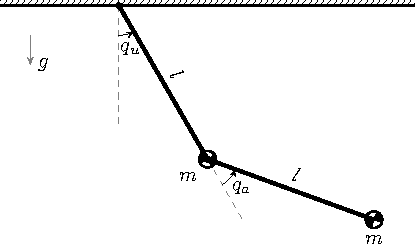
\includegraphics[width=0.7\linewidth]{simple_acrobot_model.pdf}
    \caption{A simple acrobot has massless rods of equal length \(l\) and 
    equal masses \(m\) at the tips.}
    \label{fig:simple-acrobot-model}
\end{figure}

The acrobot has inertia matrix 
\(M\), potential function \(V\) (with respect to
the horizontal bar), and input matrix \(B\) given as follows:
\begin{align}\label{eqn:acrobot-inertia}
    M(q) &= \begin{bmatrix}
        ml^2\left(3+2\cos(q_a)\right) & 
        ml^2\left(1+\cos(q_a)\right) \\
        ml^2\left(1+\cos(q_a)\right) &
        ml^2
    \end{bmatrix} 
    , \\
    \label{eqn:acrobot-potential}
    V(q) &= -mgl\left(2\cos(q_u)+\cos(q_u+q_a)\right)
    , \\
    \label{eqn:acrobot-B}
    B &= [0;1]
    .
\end{align}
The conjugate of momenta is \(p = (p_u,p_a) = M(q)\dot{q}\).
The dynamics of the acrobot in \((q,p)\) coordinates are given in
~\eqref{eqn:acrobot-hamiltonian}, where
for shorthand, we write \(c_u := \cos(q_u)\), \(c_a := \cos(q_a)\), and 
\(c_{ua} := \cos(q_u + q_a)\); likewise, \(s_u := \sin(q_u)\), 
\(s_a := \sin(q_a)\), and \(s_{ua} := \sin(q_u + q_a)\).
\begin{align}\label{eqn:acrobot-hamiltonian}
    \mathcal{H}(q,p) &= \frac{1}{2}p\tpose \Minv(q) p -
    mgl\left(2 c_u + c_{ua}\right)
    , \\
     &\begin{cases}
        \dot{q} = \Minv(q) p 
        ,\\
        \dot{p}_u = -mgl\left(2s_u + s_{ua}\right) 
        ,\\
        \dot{p}_a =-\frac{1}{2}p\tpose \nabla_{q_a}\Minv(q) p
        - mgl s_{ua} + \tau,
    \end{cases} \nonumber
\end{align}
The control input is a force \(\tau \in \R\) affecting only the dynamics of
\(p_a\), representing a torque acting on the hip joint.
This means \((q,p)\) are simply actuated coordinates inside the phase space
\(\mathcal{Q} \times \mathcal{P}\) where
\(\mathcal{Q} = \Sone \times \Sone\), and
\(\mathcal{P} = \R \times \R\).
We can therefore apply the theory of VNHCs from Section \ref{sec:vnhc} to design
a constraint of the form \(q_a = f(q_u,p_u)\). 
This constraint must inject energy into the acrobot according to
Definition \ref{defn:energy-injection}.
Since we need the VNHC to be regular, the following proposition will prove
useful.
\begin{prop}\label{prop:acrobot-fpu-regular}
    A relation \(h(q,p) = q_a - f(p_u) = 0\) 
    with \(f \in C^2\left(\R; \Sone\right)\) is a regular
    VNHC of order 1 for the simple acrobot.
\end{prop}
\begin{proof}
    The regularity matrix for this VNHC evaluates to
    \(\frac{(1+c_a)\partial_{q_u}f(q_u,p_u) + (3+2c_a)}{ml^2(2-c_a^2)}\).
    Since \(\partial_{q_u} f = 0\), this matrix is strictly positive for all values
    of \(q_a\), and hence is full rank everywhere on the constraint manifold.
\end{proof}

To design our VNHC, we begin by examining a person on a
seated swing.
The person extends their legs when the swing moves forwards, and retracts their
legs when the swing moves backwards.
As the swing gains speed, the person leans their body back while
extending their legs higher, thereby shortening the distance
from their center of mass to the pivot and adding more energy to the swing
\cite{how_to_pump_a_swing}.

Now imagine the person's torso is affixed to the swing's rope so they are
always upright. 
Imagine further that the swing has no seat at all, allowing the person to extend
their legs beneath them. 
This position is identical to that of a gymnast on a bar.

The acrobot's legs are rigid rods which cannot retract, so we emulate the person
on a swing by pivoting the legs toward the direction of motion. 
Since a person lifts their legs higher at higher speeds, the acrobot's legs should
pivot to an angle proportional to the swing's speed.
Because the direction of motion is entirely determined by \(p_u\), 
one VNHC which emulates this process is \(q_a = \bar{q}_a\arctan( I p_u)\),
displayed in Figure \ref{fig:qa-arctan}.
Here, \(\bar{q}_a \in \, ]0,2 Q_a/\pi]\) is constant and \(I \in \R\) is a fixed
control parameter.

This constraint does not perfectly recreate giant motion, during which
the gymnast's legs are almost completely extended \cite{usagym_giant}:
it instead pivots the legs partially during rotations.
However, the behaviour looks similar enough that this constraint should 
still inject energy into the acrobot.
Our final VNHC is
\begin{equation}\label{eqn:acrobot-constraint}
    h(q,p) = q_a - \bar{q}_a \arctan(I p_u)
    .
\end{equation}

\begin{figure}
    \centering
    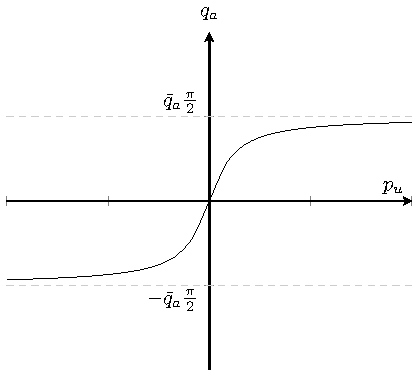
\includegraphics[width=0.7\linewidth]{qa_arctan.pdf}
    \caption{The acrobot constraint \(q_a = \bar{q}_a \arctan(I p_u)\).}
    \label{fig:qa-arctan}
\end{figure}

Recall that \((q_u, p_u)\) denote the angle and momentum of the acrobot's torso.
By Theorem \ref{thm:zero-dynamics}, we can study the constrained system by
examining solely the motion of \((q_u,p_u) \in \SxR\).
It is easy to show that the constrained dynamics are
\begin{equation}\label{eqn:acrobot-constrained-dynamics}
    \begin{cases}
    \dot{q}_u &= \frac{(1+I^2 p_u^2)p_u + m^2gl^3\bar{q}_a I(2s_u + s_{ua})(1+c_a) }
            {ml^2(1+I^2 p_u^2)(3+2c_a)}
    ,    \\
    \dot{p}_u &= - m g l (2s_u + s_{ua})
    ,
    \end{cases}
\end{equation}
subject to \(q_a = \bar{q}_a \arctan(I p_u)\).
These are just the torso dynamics when one swings the legs
according to \eqref{eqn:acrobot-constraint}.

Suppose for a moment that \(I = 0\), i.e.~that the legs stay fully extended.
The acrobot becomes a nominal pendulum with two masses, whose total mechanical
energy is
\begin{equation}\label{eqn:acrobot-energy}
    E(q_u,p_u) := \frac{p_u^2}{10ml^2} + 3mgl(1 - \cos(q_u))
    .
\end{equation}
The upright equilibrium of this pendulum is located at \((q_u,p_u) = (\pi,0)\).
Imagine the pendulum hits the bottom of the swing arc with momentum 
\(p_u \neq 0\). 
To reach the upright equilibrium, this momentum must be
\(p_u = \pm\sqrt{60m^2gl^3}\) because \(E(\pi,0) = E(0,\pm\sqrt{60m^2gl^3})\).
If the momentum is smaller in magnitude, the acrobot will oscillate; 
if it is larger, the pendulum will rotate around the bar.

When the pendulum is oscillating, its phase \((q_u,p_u)\) lies in the set
\begin{equation}\label{eqn:oscillation-domain}
    \mathcal{O}_1 := \left\{(q_u,p_u) \in \SxR 
    \mid E(q_u,p_u) < E(\pi,0) \right\}
    ,
\end{equation}
which is shown in Figure \ref{fig:acrobot-oscillation-domain}.
If for some \(I \neq 0\) our VNHC injects energy into the acrobot on 
\(\mathcal{O}_1\), and the constrained dynamics escape
\(\mathcal{O}_1\) in finite time, then the acrobot is guaranteed to perform
giant-like motion and begin rotating around the bar.

When the pendulum is rotating with bounded momentum
\(\abs{p_u} < \bar{\rho}\) (for some chosen \(\bar{\rho}\)),
the phase must lie inside the rotation domain
\begin{multline}\label{eqn:rotation-domain}
    \mathcal{R}(\rho) := \left\{
        (q_u,p_u) \in \SxR \mid\right.
        \\
        \left.E(\pi,0) < E(q_u,p_u) < E(0,\rho)
    \right\}
    .
\end{multline}
Connecting the regions \eqref{eqn:oscillation-domain} and
\eqref{eqn:rotation-domain} yields the set
\begin{equation}\label{eqn:o-rhobar}
    \mathcal{O}_2(\bar{\rho}) := \left\{(q_u,p_u) \in \SxR
        \mid E(q_u,p_u) < E(0,\bar{\rho}) \right\}
    ,
\end{equation}
shown in Figure \ref{fig:acrobot-o2}.
If the VNHC injects energy on \(\mathcal{O}_2(\bar{\rho})\) for some 
\(I \neq 0\), then the acrobot must necessarily swing up, begin rotating, 
and eventually rotate with a momentum of at least \(\bar{\rho}\).

\begin{figure}
    \centering
    \begin{subfigure}[t]{0.45\linewidth}
        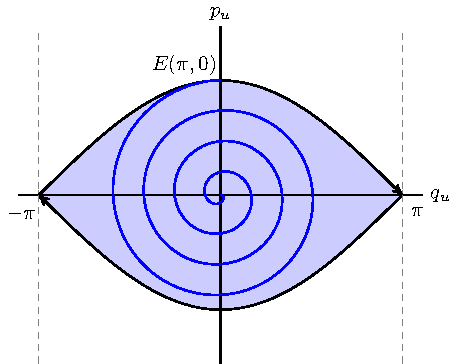
\includegraphics[width=\linewidth]{acrobot_oscillation_domain.pdf}
        \caption{The set \(\mathcal{O}_1\). An orbit starting in this set (blue)
            will pass through the level set \(E(\pi,0)\) of the nominal pendulum.}
        \label{fig:acrobot-oscillation-domain}
    \end{subfigure}
    \hfill
    \begin{subfigure}[t]{0.45\linewidth}
        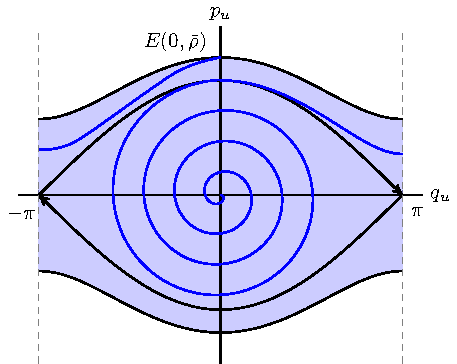
\includegraphics[width=\linewidth]{acrobot_omega.pdf}
        \caption{The set \(\mathcal{O}_2(\bar{\rho})\). Orbits starting in this
            set are guaranteed to reach the level set \(E(0,\bar{\rho})\) of the
            nominal pendulum.}
            \label{fig:acrobot-o2}
    \end{subfigure}
    \caption{The sets on which the acrobot gains energy, according to Theorem
        \ref{thm:acrobot-energy-stabilization}.}
\end{figure}

Unfortunately, our VNHC does not always inject energy on \(\mathcal{O}_1\) and
\(\mathcal{O}_2(\bar{\rho})\).
If \(I\) is too large, the leg controller saturates (i.e. the legs swing up too
quickly) and the body may not swing higher. 
However, choosing \(I\) small enough guarantees the legs will synchronize
properly with the body, and the acrobot will begin doing backflips on the bar.
The following theorem provides conditions under which such an \(I\) exists.

\begin{thm}\label{thm:acrobot-energy-stabilization}
    Consider the acrobot with Hamiltonian dynamics, as in ~\eqref{eqn:acrobot-hamiltonian}.
\begin{enumerate}
    \item For any \(m\), \(g\), \(l\), \(\bar{q}_a\), there exists
        \(I^\star > 0\) such that, for all \(I \in \, ]0,I^\star]\), the VNHC
        ~\eqref{eqn:acrobot-constraint} injects energy into the acrobot on
        \(\mathcal{O}_1\).
        Moreover, almost every orbit will escape the closure of
        \(\mathcal{O}_1\) in finite time.
        If instead \(I \in [-I^\star,0[\), the VNHC dissipates energy.
    \item Let \(C = m^2gl^3\bar{q}_a\) and 
        define \(b : \SxR_{> 0} \rightarrow \R\) by
    \[
        b(\beta,\rho_0) := 
        \frac{5C \left(
        \frac{C}{\bar{q}_a}\left(18s_\beta^2 + 30c_\beta(1 - c_\beta)\right)
            - c_\beta\rho_0^2
        \right)}{
        |\rho_0|\sqrt{\rho_0^2 - 30m^2gl^3(1 - c_\beta)}
        }
        .
    \]
        Define 
        \(S(\rho_0) := \int \limits_{0}^{2\pi} b(\sigma,\rho_0)d\sigma\).
        Fix \(\bar{\rho} > \sqrt{60m^2gl^3}\) and
        suppose there exists \(\epsilon > 0\) so that 
        \(S(\rho_0) \geq \epsilon\) for all 
        \(\rho_0 \in \, \left]\sqrt{60m^2gl^3}, \bar{\rho}\right]\).
        Then there exists \(I^{\star\star} \in \, ]0, I^\star]\) such that, for all 
        \(I \in \, ]0,I^{\star\star}]\), the VNHC
        ~\eqref{eqn:acrobot-constraint} injects energy into the acrobot on
        \(\mathcal{O}_2(\bar{\rho})\).
        If instead \(I \in [-I^{\star\star},0[\), the VNHC dissipates energy.
\end{enumerate}
\end{thm}
\begin{proof}
    See Section \ref{sec:proof}.
\end{proof}

Notice that \(\mathcal{O}_1 \subset \mathcal{O}_2(\bar{\rho})\), yet
Theorem \ref{thm:acrobot-energy-stabilization} considers these sets separately.
This separation is advantageous because the first result holds for any
\(m\), \(g\), \(l\), and \(\bar{q}_a\). 
In other words, the first result of Theorem
\ref{thm:acrobot-energy-stabilization} states that all acrobots constrained by
~\eqref{eqn:acrobot-constraint} will gain enough energy to begin rotating around
the bar.
In the worst case, the acrobot will at least perform a swing-up routine to reach
the unstable equilibrium at \((q_u,p_u) = (\pi,0)\).

For the acrobot to achieve giants with energy
\(E(0,\bar{\rho})\), it must satisfy the assumption on the integral
of \(b(\beta,\rho_0)\). 
The value of this integral depends on the acrobot's physical parameters.
If the assumption holds, there is some control value \(I > 0\)
(which depends on \(\bar{\rho}\)) for which the acrobot will 
achieve rotations with a momentum of at least \(\bar{\rho}\).

%/========== Experiments ==========/%
\section{Experimental Results}\label{sec:experiments}
In this section, we test our VNHC on the physical acrobot built by
Xingbo Wang \cite{xingbo_thesis} (Figure \ref{fig:xingbo-acrobot}).
The torso and leg rods on this robot have unequal mass and differ in length, so
its inertia matrix and potential function are not described correctly by 
~\eqref{eqn:acrobot-inertia}-\eqref{eqn:acrobot-potential}.
These experiments will therefore show that VNHCs are robust to model mismatch.

\begin{figure}
    \centering
    %\includegraphics[width=0.5\linewidth]{}
    \caption{\textbf{TODO: take a square photo of the acrobot}The acrobot built by Wang \cite{xingbo_thesis}.}
    \label{fig:xingbo-acrobot}
\end{figure}


The control parameter \(I\) must be small to satisfy Theorem
\ref{thm:acrobot-energy-stabilization}, but it must also be large enough to
overcome friction in the servo motor.
We experimentally determined that \(I = 10\) is sufficient to
ensure the actuator can fully rotate in its allowable range
\(q_a \in \left[ -\frac{\pi}{2}, \frac{\pi}{2}\right]\).

\subsection{Simulations Results}
Evaluating the true mechanical energy of Wang's acrobot at the VNHC
\(q_a = 0\) yields the energy of the nominal pendulum,
\[
    E(q_u,p_u) \approx 396.5501 p_u^2 + 0.5997(1 - \cos(q_u))
    .
\]
We simulated Wang's acrobot starting at 
\((q_u,p_u) = \left(\frac{\pi}{32},0 \right)\) and plotted the resulting orbit
in Figure \ref{fig:acrobot-orbit}.

The set \(E_\pi := E(\pi,0)\) is outlined in black. 
Because of model mismatch, \(E_\pi\) is no longer the boundary between
rotations and oscillations.
The oscillation domain is actually much larger: orbits rotate once they hit the
\(p_u\)-axis at \(\abs{p_u} \approx 0.15\), while \(E_\pi\) intersects the
\(p_u\)-axis at \(\abs{p_u} \approx 0.055\).
Despite this, the VNHC still injects energy into the acrobot.
The points where the orbit exits \(E_\pi\) are marked with black stars,
with the final departure marked with a red star.
After this final departure, the acrobot begins rotating and continues to gain
energy over time.

\begin{figure}[h]
    \centering
    \begin{subfigure}[t]{0.45\linewidth}
        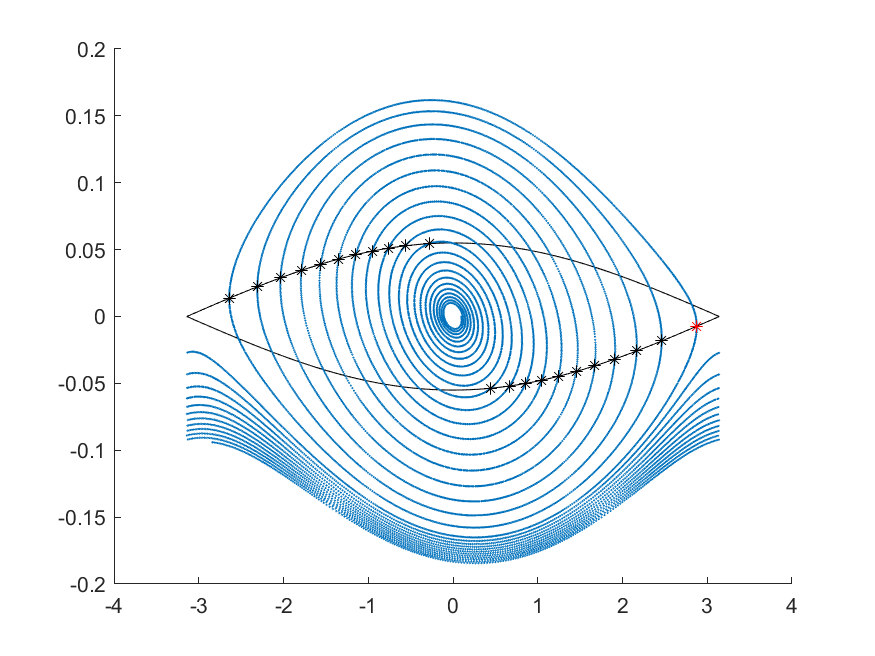
\includegraphics[width=\linewidth]{acrobot_orbit.png}
        \caption{Orbit initialized at \((q_u,p_u) = (\pi/32,0)\).}
        \label{fig:acrobot-orbit}
    \end{subfigure}
    \begin{subfigure}[t]{0.45\linewidth}
        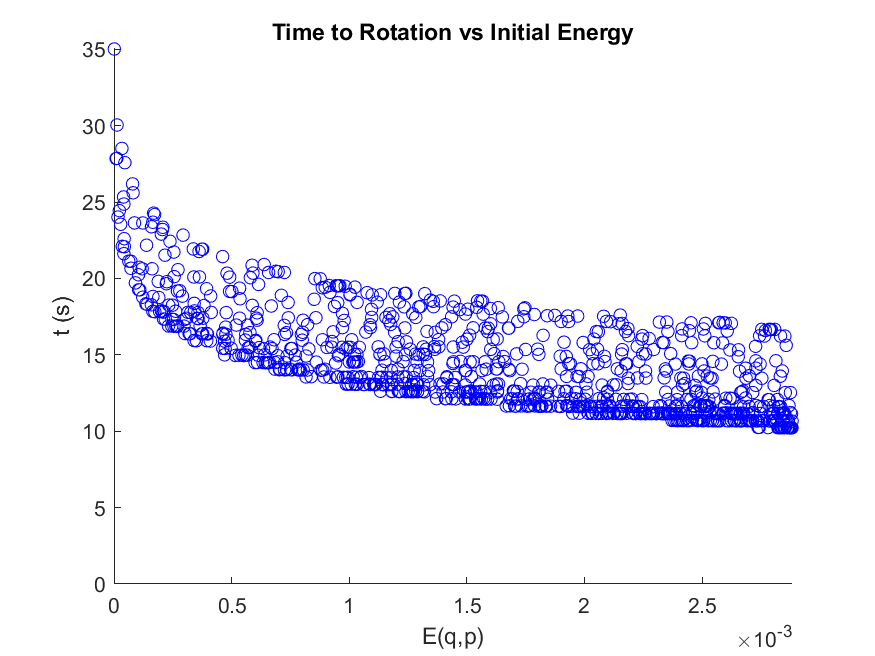
\includegraphics[width=\linewidth]{acrobot_mc.png}
        \caption{Monte Carlo results.}
        \label{fig:acrobot-mc}
    \end{subfigure}
    \caption{Simulations using Wang's acrobot \cite{xingbo_thesis}.}
\end{figure}


To verify that the acrobot would always achieve rotations, we ran a
Monte-Carlo simulation \cite{montecarlo}:
we initialized the acrobot randomly inside the sublevel set
\[
    \left\{(q_u,p_u) \in \SxR \mid
    E(q_u,p_u) \leq E\left(\frac{\pi}{32},0\right)\right\}
    ,
\] 
and measured the how long it took to begin rotating.
The results in Figure \ref{fig:acrobot-mc} show that
the acrobot always rotated within 10--35 seconds.

\subsection{Physical Experiments}
Wang's acrobot has an encoder at the pivot which measures \(q_u\) and
\(\dot{q}_u\).
The leg actuator is a servo motor with a built-in PID controller, which provides
measurements of \(q_a\).
We estimate \(\dot{q}_a\) through sequential values of \(q_a\) and
compute \(p_u\) through \(p_u = e_1^T M(q) \dot{q}\).
We then assign the actuator value at iteration \(k \in \mathbb{Z}_{> 0}\)
via \(q_a^{k} = \arctan(I p_u^{k-1})\).

\textbf{Baseline Test:} 
for this test, we initialized the acrobot at 
\((q_u,p_u) \approx \left(\frac{\pi}{8},0\right)\). 
The resulting orbit is shown in Figure \ref{fig:acrobot-unperturbed-orbit};
the acrobot is clearly gaining energy over time.

\begin{figure}
    \centering
    \begin{subfigure}[t]{0.45\linewidth}
        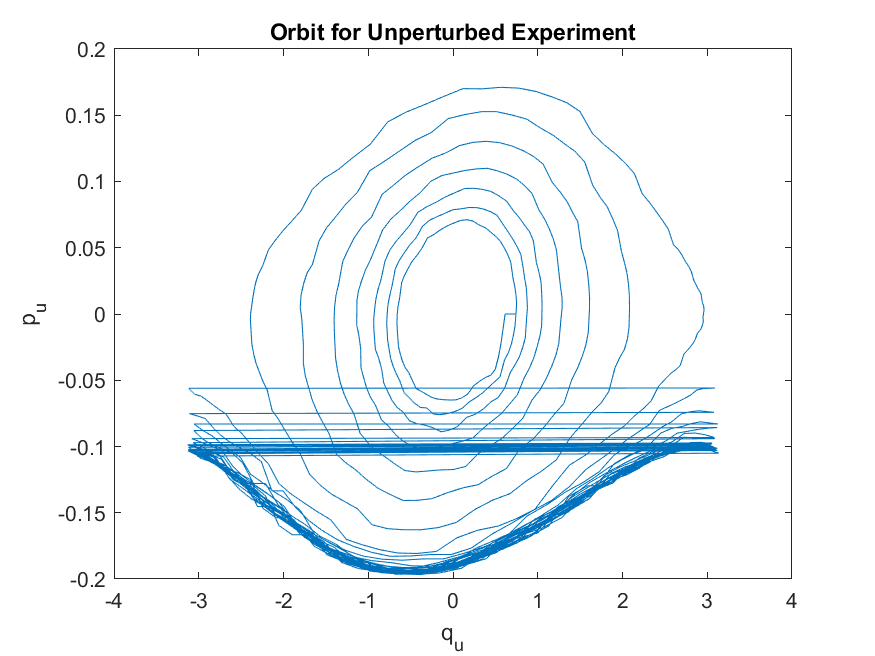
\includegraphics[width=\linewidth]{acrobot_unperturbed_orbit.png}
        \caption{The baseline test.}
        \label{fig:acrobot-unperturbed-orbit}
    \end{subfigure}
    \begin{subfigure}[t]{0.45\linewidth}
        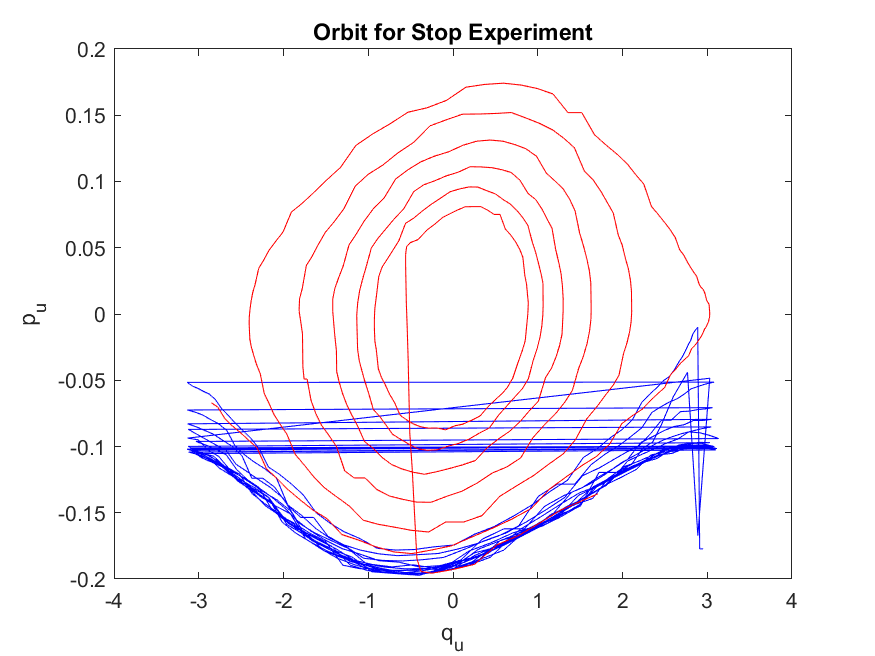
\includegraphics[width=\linewidth]{acrobot_stopped_orbit.png}
        \caption{Acrobot orbit before (blue) and after (red) stopping.}
        \label{fig:acrobot-stopped-orbit}
    \end{subfigure}
    \caption{The physical acrobot's orbit during baseline and stop tests.}
\end{figure}

\textbf{Stop Test:}
for this test we initialized the acrobot at 
\((q_u,p_u) \approx \left(\pi,0\right)\), let it run for 15
seconds, then stopped it at the bottom of its arc.
The resulting orbit is shown in Figure \ref{fig:acrobot-stopped-orbit}.
The blue curves correspond to the orbit before the disturbance, while the red
spiral confirms that the acrobot begins oscillating after it is stopped.
Despite the disturbance, it gains energy and eventually starts rotating
again.

\textbf{Push Test:}
to see how the acrobot responds when pushed, we allowed
the acrobot to rotate undisturbed for 15 seconds and then pushed it in its
direction of motion.
The orbit in Figure \ref{fig:acrobot-fpush-orbit} shows that the acrobot speeds
up to rotate with energy \(E(0,0.22)\), but then slows down until it reaches a
stable rotation with energy \(E(0,-0.195)\).
We repeated this test by pushing the acrobot against its direction of motion.
The orbit in Figure \ref{fig:acrobot-rpush-orbit} demonstrates that the acrobot
responds by readily changing direction, and quickly achieves its maximum speed
with energy \(E(0,0.195)\).

These push tests suggest that our VNHC injects energy into Wang's acrobot on
\(\mathcal{O}_2(0.195)\).


\begin{figure}
    \centering
    \begin{subfigure}[ht]{0.45\linewidth}
        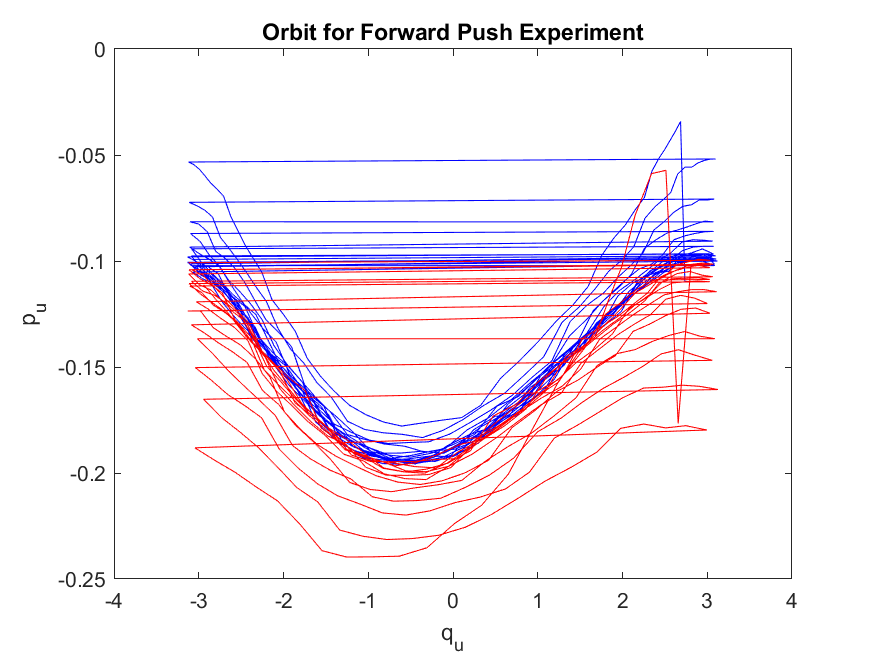
\includegraphics[width=\linewidth]{acrobot_fpush_orbit.png}
        \caption{The forwards push test.}
        \label{fig:acrobot-fpush-orbit}
    \end{subfigure}
    \begin{subfigure}[ht]{0.45\linewidth}
        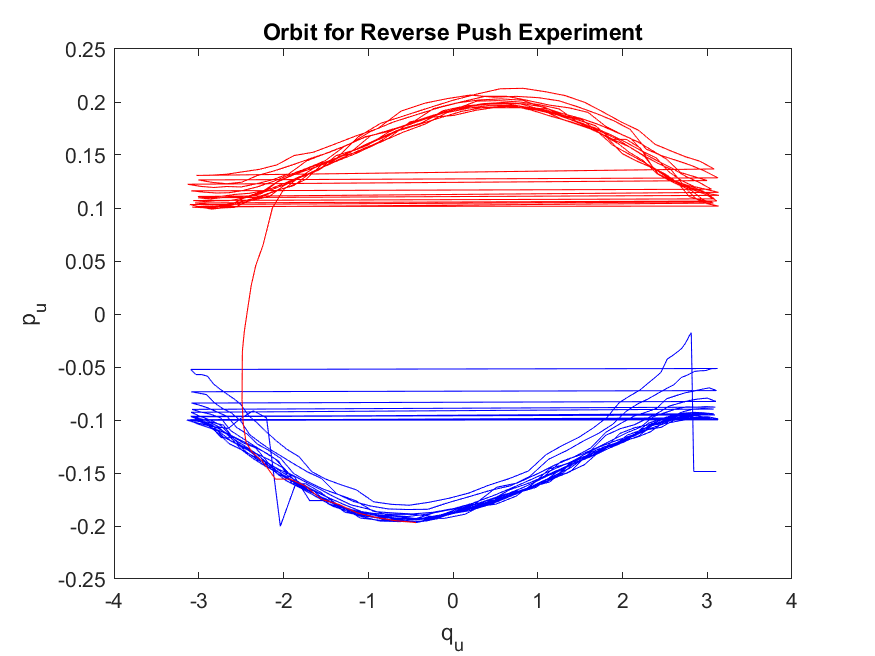
\includegraphics[width=\linewidth]{acrobot_rpush_orbit.png}
        \caption{The reverse push test.}
        \label{fig:acrobot-rpush-orbit}
    \end{subfigure}
    \caption{The acrobot orbit before (blue) and after (red) pushing.}
\end{figure}

\subsection{Summary of Experiments}
These simulations and experiments demonstrate that VNHCs are excellent
tools for injecting energy, even with significant model mismatch.
In particular, energy injection through VNHCs appears to be robust against a
variety of disturbances.

%/========== Proof ==========/%
\section{Proof of Theorem \ref{thm:acrobot-energy-stabilization}}\label{sec:proof}

%/========== Conclusion ==========/%
\section{Conclusion}\label{sec:conclusion}
In this article we summarized the existing theory of virtual nonholonomic
constraints (VNHCs) ........
\textbf{TODO conclude nicely}
In the end, we demonstrated that virtual nonholonomic constraints are capable of
injecting and dissipating energy in a robust manner, all while producing
realistic biological motion.



%---------- Bibliography ----------%
\bibliography{bib}
\end{document}
%/========== /Main Document ==========/%
% vim: set tw=80 ts=4 sw=4 sts=0 et ffs=unix :
